%%%%%%%%%%%%%%%%%%%%%%%%%%%%%%%%%%%%%%%%%%%%%%%%%%%%%%%%%%%%%%%%%%%%%%%%%%%%%%%%
%2345678901234567890123456789012345678901234567890123456789012345678901234567890
%        1         2         3         4         5         6         7         8

%\documentclass[letterpaper, 10 pt, conference]{ieeeconf}  % Comment this line out
                                                          % if you need a4paper
\documentclass[letterpaper, 10pt, conference]{ieeeconf}      % Use this line for a4
                                                          % paper

 
\IEEEoverridecommandlockouts                              % This command is only
                                                          % needed if you want to
                                                          % use the \thanks command
\overrideIEEEmargins
% See the \addtolength command later in the file to balance the column lengths
% on the last page of the document

\usepackage{amsmath}    % need for sub equations
\usepackage{amsfonts}
\usepackage{graphicx}   % need for figures
\usepackage{subcaption}
\usepackage{epsfig} 
\usepackage{cancel}
\usepackage{amssymb}
\usepackage{color}
\usepackage{my_macros}
\usepackage[ruled,vlined,titlenotnumbered]{algorithm2e} 

\title{\LARGE \bf
Safe Sequential Path Planning of Multi-Vehicle Systems via Double-Obstacle Hamilton-Jacobi-Isaacs Variational Inequality}

\author{Mo Chen, Jaime F. Fisac, Shankar Sastry, Claire J. Tomlin
\thanks{This work has been supported in part by NSF under CPS:ActionWebs (CNS-931843), by ONR under the HUNT (N0014-08-0696) and SMARTS (N00014-09-1-1051) MURIs and by grant N00014-12-1-0609, by AFOSR under the CHASE MURI (FA9550-10-1-0567). The research of J.F. Fisac has received funding from the ``la Caixa" Foundation.}
\thanks{All authors are with the Department of Electrical Engineering and Computer Sciences, University of California, Berkeley. \{mochen72, jfisac, sastry, tomlin\}@eecs.berkeley.edu}
}

\begin{document}
\maketitle
\thispagestyle{empty}
\pagestyle{empty}

%%%
\begin{abstract}
We consider the problem of planning trajectories for a group of $N$ vehicles, each aiming to reach its own target set while avoiding danger zones of other vehicles. The analysis of problems like this is extremely important practically, especially given the growing interest in utilizing unmanned aircraft systems for civil purposes. The direct solution of this problem by solving a single-obstacle Hamilton-Jacobi-Isaacs (HJI) variational inequality (VI) is numerically intractable due to the exponential scaling of computation complexity with problem dimensionality. Furthermore, the single-obstacle HJI VI cannot directly handle situations in which vehicles do not have a common scheduled arrival time. Instead, we perform sequential path planning  by considering vehicles in order of priority, modeling higher-priority vehicles as time-varying obstacles for lower-priority vehicles. To do this, we solve a double-obstacle HJI VI which allows us to obtain the reach-avoid set, defined as the set of states from which a vehicle can reach its target while staying within a time-varying state constraint set. From the solution of the double-obstacle HJI VI, we can also extract the latest start time and the optimal control for each vehicle. This is a first application of the double-obstacle HJI VI which can handle systems with time-varying dynamics, target sets, and state constraint sets, and results in computation complexity that scales linearly, as opposed to exponentially, with the number of vehicles in consideration.
\end{abstract}

% % !TEX root = ../SPP_IoTjournal.tex
\section{Introduction \label{sec:introduction}}
Recently, there has been an immense surge of interest in the use of unmanned aerial systems (UASs) for civil applications. The applications include package delivery, aerial surveillance, disaster response, among many others \cite{Tice91, Debusk10, Amazon16, AUVSI16, BBC16}. These civil applications will involve unmanned aerial vehicles (UAVs) flying in urban environments, potentially in close proximity to humans, other UAVs, and other important assets. As a result, government agencies such as the Federal Aviation Administration (FAA) and National Aeronautics and Space Administration (NASA) of the United States are urgently trying to develop new scalable ways to organize an airspace in which potentially thousands of UAVs can fly together \cite{FAA13, Kopardekar16}.

One essential problem that needs to be addressed for this endeavor to be successful is that of trajectory planning: how a group of vehicles in the same vicinity can reach their destinations while avoiding situations which are considered dangerous, such as collisions. Many previous studies address this problem under different assumptions. In some studies, specific control strategies for the vehicles are assumed, and approaches such as those involving induced velocity obstacles \cite{Fiorini98, Chasparis05, Vandenberg08,Wu2012} and involving virtual potential fields to maintain collision avoidance \cite{Olfati-Saber2002, Chuang07} have been used. Methods have also been proposed for real-time trajectory generation \cite{Feng-LiLian2002}, for path planning for vehicles with linear dynamics in the presence of obstacles with known motion \cite{Ahmadzadeh2009}, and for cooperative path planning via waypoints which do not account for vehicle dynamics \cite{Bellingham}. Other related work is in the collision avoidance problem without path planning. These results include those that assume the system has a linear model \cite{Beard2003, Schouwenaars2004, Stipanovic2007}, rely on a linearization of the system model \cite{Massink2001, Althoff2011}, assume a simple positional state space \cite{Lin2015}, and many others \cite{Lalish2008, Hoffmann2008, Chen2016}.

However, to make sure that a dense group of UAVs can safely fly in close vicinity of each other, we need the capability to flexibly plan provably safe and dynamically feasible trajectories without making strong assumptions on the vehicles' dynamics and other vehicles' motion. Moreover, any trajectory planning scheme that addresses collision avoidance must also guarantee both goal satisfaction and safety of UAVs despite disturbances caused by wind and communication faults \cite{Kopardekar16}. Furthermore, unexpected scenarios such as UAV malfunctions or even UAVs with malicious intent need to be accounted for. Finally, the proposed scheme should scale well with the number of vehicles.

The problem of trajectory planning and collision avoidance under disturbances in safety-critical systems has been studied using Hamilton-Jacobi (HJ) reachability analysis, which provides guarantees on goal satisfaction and safety of optimal system trajectories \cite{Barron90, Mitchell05, Bokanowski10, Bokanowski11, Margellos11, Fisac15}. Reachability-based methods are particularly suitable in the context of UAVs because of the formal guarantees that are provided. In reachability analysis, one computes the reach-avoid set, defined as the set of states from which the system can be driven to a target set while satisfying time-varying state constraints at all times. A major practical appeal of this approach stems from the availability of modern numerical tools, which can compute various definitions of reachable sets \cite{Sethian96, Osher02, Mitchell02, Mitchell07b}. These numerical tools, for example, have been successfully used to solve a variety of differential games, trajectory planning problems, and optimal control problems. Concrete practical applications include aircraft auto-landing \cite{Bayen07}, automated aerial refueling \cite{Ding08}, MPC control of quadrotors \cite{Bouffard12}, and multiplayer reach-avoid games \cite{Huang11}. Despite its power, the approach becomes numerically intractable as the state space dimension increases. In particular, reachable set computations involve solving a HJ partial differential equation (PDE) or variational inequality (VI) on a grid representing a discretization of the state space, resulting in an \textit{exponential} scaling of computational complexity with respect to the dimensionality of the problem. Therefore, as such, dynamic programming-based approaches such as reachability analysis are not suitable for managing the next generation airspace, which is a large-scale system with a high-dimensional joint state space because of the possible high density of vehicles that needs to be accommodated \cite{Kopardekar16}.  

To overcome this problem, the Sequential Path Planning (SPP) method has been proposed \cite{Chen15c}, in which vehicles are assigned a strict priority ordering. Higher-priority vehicles plan their trajectories without taking into account the lower-priority vehicles. Lower-priority vehicles treat higher-priority vehicles as moving obstacles. Under this assumption, time-varying formulations of reachability \cite{Bokanowski11, Fisac15} can be used to obtain the optimal and provably safe trajectories for each vehicle, starting from the highest-priority vehicle. Thus, the curse of dimensionality is overcome for the multi-vehicle trajectory planning problem at the cost of a structural assumption, under which the computation complexity scales just \textit{linearly} with the number of vehicles. In addition, a structure like this has the potential to flexibly divide up the airspace for the use of many UAVs and allows a tractable multi-vehicle trajectory-planning. In general, different economic mechanisms can be used to come up with a priority order. One example could be first-come-first-serve mechanism, as highlighted in NASA’s concept of operations for UAS traffic management \cite{Kopardekar16}. \SBnote{Mo, could you please read this paragraph again?}

The authors in \cite{Bansal2017} extend the SPP method to the scenarios where disturbances, such as wind, are present in the system, resolving some of the practical challenges associated with the basic SPP algorithm in \cite{Chen15c}. However, if a vehicle not in the set of SPP vehicles enters the system, or even worse, if this vehicle has malicious intent, the original plan can lead to vehicles entering into another vehicle’s danger zone. Thus, if vehicles do not plan with an additional safety margin that takes a potential intruder into account, a vehicle trying to avoid the intruder may effectively become an intruder itself, leading to a domino effect, causing the entire SPP structure to collapse. 

The authors in \cite{chen2016robust} propose an SPP algorithm that accounts for such a potential intruder. However, a new full-scale trajectory planning problem is required to be solved in real time to ensure safe transit of the vehicles to their respective destinations. Since the replanning must be done in real-time, the proposed algorithm is intractable for large-scale systems even with the SPP structure, rendering the method unsuitable for practical implementation in these cases. In this work, we propose a novel intruder avoidance algorithm, which will need to replan trajectories only for a \textit{fixed number of vehicles} if the intruder appears in the system, irrespective of the total number of SPP vehicles. Moreover, this number is a design parameter, which can be chosen beforehand based on the computational resources available for replanning during the run time, thus overcoming the limitations of the algorithm in \cite{chen2016robust}. 

Intuitively, for every vehicle, we compute a \textit{separation region} such that the vehicle needs to account for the intruder if and only if the intruder is inside this separation region. We then compute a \textit{buffer region} between the separation regions of any two vehicles, and ensure that this buffer is maintained as vehicles are traveling to their destinations. Thus, to intrude with any additional vehicle, the intruder will have to travel through this buffer region. In fact, we can affect this traveling time based on the size of the buffer region. Thus, for a given time duration, we can design the buffer region size such that the intruder can affect atmost a desirable number of vehicles. A high-level overview of the proposed algorithm is provided in Algorithm \ref{alg:basic_idea}.    
%
\begin{algorithm}[tb]
\SetKwInOut{Input}{input}
\SetKwInOut{Output}{output}
	\DontPrintSemicolon
	\caption{Overview of the proposed intruder avoidance algorithm (planning phase)}
	\label{alg:basic_idea}
	\Input{Set of vehicles $\veh_i, i = 1, \ldots, \N$ in the descending priority order;\newline
	Vehicle dynamics and initial states;\newline
	Vehicle destinations and any obstacles to avoid;\newline
	Intruder dynamics;\newline
	$\nva$: Maximum number of vehicles allowed to re-plan their trajectories.}
    \Output{Provably safe vehicle trajectories to respective destinations despite disturbance and intruder;\newline 
    Intruder avoidance and goal-satisfaction controller.}
	\For{\text{$i=1:N$}}{
			compute the separation region of $\veh_i$;\;
			compute the required buffer region based on $\nva$;\;
			use SPP algorithm for trajectory planning of $\veh_i$ such that the buffer region is maintained between $\veh_i$ and $\veh_j$ for all $j<i$;\;
			output the trajectory and optimal controller for $\veh_i$.\;
		}
\end{algorithm}
%

The rest of the paper is organized as follows: in Section \ref{sec:formulation}, we formally present the SPP problem in the presence of disturbances and adversarial intruders. In Section \ref{sec:background}, we present a brief review of time-varying reachability and the basic SPP algorithms proposed in \cite{Chen15c}, \cite{Bansal2017}. In Section \ref{sec:intruder}, we explain the proposed algorithm to account for intruders. Finally, we illustrate this algorithm through a fifty-vehicle simulation in an urban environment in Section \ref{sec:simulations}. All running notations in this paper are summarized in Table \ref{table:notation}.
% Introduction (1-1.5p)
%% Motivation
%% Related work
%% Summary of results
\section{Introduction}
Consider a group of autonomous vehicles trying to perform a task or reach a goal which may be time-varying in their joint state space, while avoiding obstacles and other vehicles. Providing safety and performance guarantees for such a multi-agent autonomous system (MGAS) is very relevant practically. Unmanned aerial vehicles (UAVs), for example, have in the past been used mainly for military operations \cite{tice91}. However, recently, there has been a growing interest in using UAVs for civil applications, as companies like Amazon and Google are looking in the near future to send UAVs into the airspace to deliver packages \cite{primeAir,projectWing}. Government agencies such as the Federal Aviation Administration (FAA) and National Aeronautics and Space Administration (NASA) of the United States are also expressing growing interest in analyzing these problems in order to prevent airspace conflicts that could arise with the introduction of potentially many UAVs in an urban environment \cite{faa13}. In addition, UAVs can be used not only to deliver packages quickly, but in any situation where fast response is desired. For example, UAVs can provide emergency supplies to disaster-struck areas that are otherwise difficult to reach \cite{debusk10}.

In general, MGASs are difficult to analyze due to their inherent high dimensionality. For example, the joint state space of 10 vehicles would have 30 dimensions even if each vehicle is described by a simple model with three states. MGASs also often involve aspects of cooperation and asymmetric goals among the vehicles or teams of vehicles, making their analysis particularly interesting. Despite these difficulties, it is still important to analyze these systems because of their applications in robotics and aircraft safety.

MGASs have been explored extensively in the literature. Some researchers have done work on multi-vehicle path planning in the presence of other unknown vehicles or moving entities with assumptions on their specific control strategies \cite{chasparis05}. In a number of formulations for safe multi-vehicle navigation, these assumed strategies induce velocity obstacles that vehicles must avoid to maintain safety \cite{fiorini98, vandenberg08}. Researchers have also used potential functions to perform collision avoidance while maintaining formation given a predefined trajectory \cite{saber02,chuang07}. However, these bodies of work have not considered trajectory planning and collision avoidance simultaneously.

One well-known technique for optimal trajectory planning under disturbances or adversaries is reachability analysis, in which one computes the reach-avoid set, defined as the set of states from which the system can reach a target set while remaining within a state constraint set for all time. For reachability of systems of up to five dimensions, single-obstacle Hamilton-Jacobi-Isaacs (HJI) variational inequalities (VI) \cite{mitchell05,bokanowski10} have been used in situations where obstacles and target sets are static. Another HJI VI formulation \cite{barron89} is able to handle problems with moving target sets with no obstacles. 

A major practical appeal of the above approaches stems from the availability of modern numerical tools such as \cite{mitchell05, sethian96, osher02, LSToolbox}, which can efficiently solve HJI equations when the problem dimension is low. These numerical tools have been successfully used to solve a variety of differential games, path planning problems, and optimal control problems, including aircraft collision avoidance \cite{mitchell05}, automated in-flight refueling \cite{ding08}, and two-player reach-avoid games \cite{huang11}. The advantage of the HJI approaches is that they can be applied to a large variety of system dynamics, and provide guarantees on the system's safety and performance.

Despite the power of the previous HJI formulations, the approaches become numerically intractable very quickly as the number of vehicles in the system is increased. This is because the numerical computations are done on a grid in the joint state space of the system, resulting in an exponential scaling of computation complexity with respect to the dimensionality of the problem. Furthermore, state constraint sets, while useful for modeling unsafe vehicle configurations, are required to be time-invariant in \cite{mitchell05, bokanowski10, mitchell-thesis}. To solve problems involving time-varying state constraints, \cite{bokanowski11} proposed to augment the state space with time; however, this process introduces an extra state space dimension without addressing the added computation complexity.

Recently, \cite{fisac15} presented a double-obstacle HJI VI which handles problems in which the dynamics, target sets, and state constraint sets are all time-varying, and provided a numerical implementation based on well-known schemes. The formulation does not introduce any additional computation overhead compared to the above-mentioned techniques, yet it still maintains the same guarantees on the system's safety and performance. In this paper, we provide a first application of the theory presented in \cite{fisac15}. As a point of clarification, ``obstacles" in the context of HJI VIs refer to the effective constraints in the HJI VI, while obstacles in the state space represent physical obstacles that vehicles must avoid.

Our contributions are as follows. First, we formulate a multi-vehicle collision avoidance problem involving $N$ autonomous vehicles. Each vehicle seeks to get to its own target sets while avoiding obstacles and collision with all other vehicles. To reduce the problem complexity to make the problem tractable, we assign a priority to each vehicle, and model higher-priority vehicles as time-varying obstacles that need to be avoided. We then utilize the double-obstacle HJI VI proposed in \cite{fisac15} to compute reach-avoid sets to plan trajectories for vehicles in order of priority. This way, we are able to offer a tractable solution that scales linearly, as opposed to exponentially, with the number of vehicles. We compare our approach to the previous single-obstacle HJI VI approach involving static obstacles \cite{mitchell05, bokanowski10, mitchell-thesis} in a simple two-vehicle system, and demonstrate the scalability of our approach in a more complex four-vehicle system.

% % !TEX root = ../SPP_IoTjournal.tex
\section{Sequential Path Planning Problem \label{sec:formulation}}
Consider $\N$ vehicles $\veh_i, i = 1, \ldots, \N$ (also denoted as \textit{SPP vehicles}) which participate in the SPP process. We assume their dynamics are given by

\begin{equation}
\label{eq:dyn}
\begin{aligned}
\dot\state_i &= \fdyn_i(\state_i, \ctrl_i, \dstb_i), t \le \sta_i \\
\ctrl_i &\in \cset_i, \dstb_i \in \dset_i, i = 1 \ldots, \N
\end{aligned}
\end{equation}

\noindent where $\state_i \in \R^{n_i}$, $\ctrl_i \in \cset_i$ and $\dstb_i \in \dset_i$, respectively, represent the state, control and disturbance experienced by vehicle $\veh_i$. We partition the state $\state_i$ into the position component $\pos_i \in \R^{n_\pos}$ and the non-position component $\npos_i \in \R^{n_i - n_\pos}$: $\state_i = (\pos_i, \npos_i)$. %We assume that the control functions $\ctrl_i(\cdot), \dstb_i(\cdot)$ are drawn from the set of measurable functions\footnote{A function $f:X\to Y$ between two measurable spaces $(X,\Sigma_X)$ and $(Y,\Sigma_Y)$ is said to be measurable if the preimage of a measurable set in $Y$ is a measurable set in $X$, that is: $\forall V\in\Sigma_Y, f^{-1}(V)\in\Sigma_X$, with $\Sigma_X,\Sigma_Y$ $\sigma$-algebras on $X$,$Y$.}. For convenience, 
We will use the sets $\cfset_i, \dfset_i$ to respectively denote the set of functions from which the control and disturbance functions $\ctrl_i(\cdot), \dstb_i(\cdot)$ are drawn.

% We further assume that the flow field $\fdyn_i: \R^{n_i}\times\cset_i\times\dset_i \rightarrow \R^{n_i}$ is uniformly continuous, bounded, and Lipschitz continuous in $\state_i$ for fixed $\ctrl_i$ and $\dstb_i$. With this assumption, given $\ctrl_i(\cdot) \in \cfset_i, \dstb_i(\cdot) \in \dfset_i$, there exists a unique trajectory solving \eqref{eq:dyn} \cite{EarlA.Coddington1955}. %We will denote trajectories of \eqref{eq:dyn} starting from state $\state^0_i$ at time $t_0$ under control $\ctrl_i(\cdot)$ and disturbance $\dstb_i(\cdot)$ as $\traj_i(t; \state^0_i, t_0, \ctrl_i(\cdot))$. Trajectories satisfy an initial condition and the differential equation \eqref{eq:dyn} almost everywhere:

%\begin{equation}
%\begin{aligned}
%\frac{d}{dt}\traj_i(t; \state^0_i, t_0, \ctrl_i(\cdot)) &= \fdyn(\state^0_i, \ctrl_i, \dstb_i) \\
%\traj_i(t_0; \state^0_i, t_0, \ctrl_i(\cdot)) &= \state^0_i
%\end{aligned}
%\end{equation}

%In addition, we assume that the disturbances $\dstb_i(\cdot)$ are drawn the set of non-anticipative strategies \cite{Mitchell05} $\Gamma$, defined as follows:
%\begin{equation}
%\begin{aligned}
%& \Gamma := \{\mathcal{N}: \cfset_i \rightarrow \dfset_i:  \ctrl_i(r) = \hat{\ctrl}_i(r) \text{ a. e. } r\in[t,s] \\
%& \Rightarrow \mathcal{N}[\ctrl_i](r) = \mathcal{N}[\hat{\ctrl}_i](r) \text{ a. e. } r\in[t,s]\}
%\end{aligned}
%\end{equation}

Each vehicle $\veh_i$ has initial state $\state^0_i$, and aims to reach its target $\targetset_i$ by some scheduled time of arrival $\sta_i$. The target in general represents some set of desirable states, for example the destination of $\veh_i$. %For most of the paper we will make the assumption that $\edt_i$ is early enough for $\veh_i$ to feasibly get to $\targetset_i$ on time; this can be done by letting $\edt_i \rightarrow -\infty$. The assumption on $\edt_i$ is merely for convenience: in situations where $\edt_i$ is $-\infty$. In some situations, we may find that it is infeasible for $\veh_i$ to get to $\targetset_i$ at or before $\sta_i$. Whenever unsure, we may first determine the earliest feasible $\sta_i$ as described in Section \ref{sec:intruder}.
On its way to $\targetset_i$, $\veh_i$ must avoid a set of static obstacles $\soset_i \subset \R^{n_i}$. The interpretation of $\soset_i$ could be any set of states that are forbidden for each SPP vehicle such as a tall building. Each vehicle $\veh_i$ must also avoid the danger zones with respect to every other vehicle $\veh_j, j\neq i$. The danger zones in general can represent any joint configurations between $\veh_i$ and $\veh_j$ that are considered to be unsafe. We define the danger zone of $\veh_i$ with respect to $\veh_j$ to be
\begin{equation} \label{eqn:danger_zone_defn}
\dz_{ij} = \{(\state_i, \state_j): \|\pos_i - \pos_j\|_2 \le \rc\}
\end{equation}
\noindent whose interpretation is that $\veh_i$ and $\veh_j$ are considered to be in an unsafe configuration when they are within a distance of $\rc$ of each other. In particular, $\veh_i$ and $\veh_j$ are said to have collided, if $(\state_i, \state_j) \in \dz_{ij}$.

In addition to the obstacles and danger zones, an intruder vehicle can also appear in the system. An intruder vehicle may have malicious intent or it can be a non-participating vehicle, which does not have malicious intent, but can accidentally cause a collision with other vehicles since it may not follow the SPP structure. This general definition of intruder allows us to develop algorithms that can also account for vehicles who are not communicating with the SPP vehicles or do not know about the SPP structure. \SBnote{Mo, could you please read this paragraph again? Also, do you think we should expand on this idea of ``non-participating" vehicles in the introduction?}

In general, the effect of an intruder on the vehicles in structured flight can be entirely unpredictable, since the intruder in principle could be adversarial in nature, and the number of intruders could be arbitrary. In particular, if the number of intruders in the system is arbitrary, a collision avoidance problem must to be solved for each SPP vehicle in the joint state-space of all intruders and the vehicle, even with the SPP structure. Therefore, to make our analysis intractable, we make the following two assumptions: \SBnote{Mo, could you please read this paragraph again?}
\begin{assumption}
\label{as:avoidOnce}
At most one intruder (denoted as $\veh_I$ here on) affects the SPP vehicles at any given time. The intruder is removed after a duration of $\iat$. 
\end{assumption}    
This assumption can be valid in situations where intruders are rare, and that some fail-safe or enforcement mechanism exists to force the intruder out of the planning space affecting the SPP vehicles. For example, when SPP vehicles are flying at a particular altitude level, the removal of the intruder can be achieved by exiting the altitude level.
 
Let the time at which intruder appears in the system be $\tsa$ and the time at which it disappears be $\tea$. Assumption \ref{as:avoidOnce} implies that $\tea \leq \tsa + \iat$. Thus, any vehicle $\veh_i$ would need to avoid the intruder $\veh_{\intr}$ for a maximum duration of $\iat$. After a duration of $\iat$, the intruder is no longer present in the system. Note that we do not pose any restriction on $\tsa$; we only assume that once the intruder appears, it stays for a maximum duration of $\iat$.
\begin{assumption}
\label{as:dynKnown}
The dynamics of the intruder are known and given by $\dot\state_\intr = f_\intr(\state_\intr, \ctrl_\intr, \dstb_\intr)$.
\end{assumption}
Assumption \ref{as:dynKnown} is required for HJ reachability analysis. In situations where the dynamics of the intruder are not known exactly, a conservative model of the intruder may be used instead. We also denote the initial state of the intruder as $\state_{\intr}^0.$ Note that $\state_{\intr}^0$ is unknown.

Given the set of SPP vehicles, their targets $\targetset_i$, the static obstacles $\soset_i$, the vehicles' danger zones with respect to each other $\dz_{ij}$, and the intruder dynamics $f_\intr(\cdot)$, our goal is as follows. For each vehicle $\veh_i$, synthesize a controller which guarantees that $\veh_i$ reaches its target $\targetset_i$ at or before the scheduled time of arrival $\sta_i$, while avoiding the static obstacles $\soset_i$, the danger zones with respect to all other vehicles $\dz_{ij}, j\neq i$, and the intruder vehicle $\veh_{\intr}$, irrespective of the control strategy of the intruder. In addition, we would like to obtain the latest departure time $\ldt_i$ such that $\veh_i$ can still arrive at $\targetset_i$ on time.

In general, the above optimal path planning problem must be solved in the joint space of all $\N$ SPP vehicles and the intruder vehicle. However, due to the high joint dimensionality, a direct dynamic programming-based solution is intractable. Therefore, the authors in \cite{Chen15c} proposed to assign a priority to each vehicle, and perform SPP given the assigned priorities. Without loss of generality, let $\veh_j$ have a higher priority than $\veh_i$ if $j<i$. Under the SPP scheme, higher-priority vehicles can ignore the presence of lower-priority vehicles, and perform path planning without taking into account the lower-priority vehicles' danger zones. A lower-priority vehicle $\veh_i$, on the other hand, must ensure that it does not enter the danger zones of the higher-priority vehicles $\veh_j, j<i$ or the intruder vehicle $\veh_{\intr}$; each higher-priority vehicle $\veh_j$ induces a set of time-varying obstacles $\ioset_i^j(t)$, which represents the possible states of $\veh_i$ such that a collision between $\veh_i$ and $\veh_j$ or $\veh_i$ and $\veh_{\intr}$ could occur.

It is straight-forward to see that if each vehicle $\veh_i$ is able to plan a trajectory that takes it to $\targetset_i$ while avoiding the static obstacles $\soset_i$, the danger zones of \textit{higher-priority vehicles} $\veh_j, j<i$, and the danger zone of the \textit{intruder} $\veh_{\intr}$ irrespective of the intruder's control policy, then the set of SPP vehicles $\veh_i, i=1,\ldots,\N$ would all be able to reach their targets safely. Under the SPP scheme, path planning can be done sequentially in descending order of vehicle priority in the state space of only a single vehicle. Thus, SPP provides a solution whose complexity scales linearly with the number of vehicles, as opposed to exponentially, with a direct application of dynamic programming approaches. 

However, when an intruder appears in the system, depending on the initial state of the intruder and its control policy, a vehicle may arrive at different states after avoiding the intruder. Therefore, a control policy that ensures a successful transit to the destination needs to account for all such possible states, which is a path planning problem with multiple initial states and a single destination, and is hard to solve in general. Thus, we divide the intruder avoidance problem into two sub-problems: (i) we first design a control policy that ensures a successful transit to the destination if no intruder appears and that successfully avoid the intruder, if it does (Algorithm \ref{alg:basic_idea}). (ii) after the intruder disappears at $\tea$, we replan the trajectories of the affected vehicles. Following the same theme and assumptions, the authors in \cite{chen2016robust} present an algorithm to avoid an intruder in SPP formulation; however, in the worst-case, the algorithm might need to replan the trajectories for \textit{all} SPP vehicles. Since the replanning is done in real-time, the method in \cite{chen2016robust} is unsuitable for practical implementation for large multi-vehicle systems. Our goal in this work is to present an algorithm that ensures that only a \textit{small and fixed} number of vehicles need to replan their trajectories, regardless of the total number of vehicles. Thus, the replanning time is constant and can be done in real time. In particular, we answer the following inter-dependent questions:
\begin{enumerate}
\item How can each vehicle guarantee that it will reach its target set without getting into any danger zones, despite no knowledge of the intruder initial state, the time at which it appears, and its control strategy?
\item How can we ensure that replanning only needs to be done for at most a fixed maximum number of vehicles after the intruder disappears from the system? \label{question2}
\item Can we choose the maximum number of the vehicles in question \ref{question2} above?
\end{enumerate}

\begin{table*}
    \caption{Different mathematical notations and their interpretation (in the alphabetical order of symbols).}    
    \resizebox{\hsize}{!}{
    \begin{tabular}{ |>{\centering\arraybackslash}m{1.5cm}| m{5cm} | m{3cm} | m{\columnwidth} |}
 %   \begin{tabular}{ | l | l | p{11cm} |}
    \hline
    \textbf{Notation} & \textbf{Description} & \textbf{Location} & \textbf{Interpretation} \\ \hline
    
    %%% Letter D %%% 
    % Disturbance
    $\dstb_i$ & Disturbance in the dynamics of vehicle $i$ & Beginning of Section \ref{sec:formulation} & -    \\ \hline   
    $\dstb_{\intr}$ & Disturbance in the dynamics of the intruder & Assumption \ref{as:dynKnown} & -    \\ \hline   
    
    %%% Letter F %%%
    % Dynamics
    $\fdyn_i$ & Dynamics of vehicle $i$ & Beginning of Section \ref{sec:formulation} & -    \\ \hline
    $f_\intr$ & Dynamics of the intruder & Assumption \ref{as:dynKnown} & -    \\ \hline
    $f_r$ & Relatiove dynamics between two vehicles & Equation \eqref{eq:reldyn} & - \\ \hline
    
    %%% Letter G %%%
    % Obstacle
    $\obsset_i(t)$ & The overall obstacle for vehicle $i$ & Equation \eqref{eq:obsseti} & The set of states that vehicle $i$ must avoid on its way to the destination. \\ \hline
    
    %%% Letter H %%%
    % Non-position state components of the vehicle
    $\npos_i$ & Non-position state component of vehicle $i$ & Beginning of Section \ref{sec:formulation} & -    \\ \hline
    
    %%% Letter K %%%
    % Number of vehicles to avoid
    $\nva$ & - & Beginning of Section \ref{sec:intruder} & The maximum number of vehicles that should apply the avoidnace maneuver or the maximum number of vehicles that we can replan trajectories for in real-time.    \\ \hline    
    
    %%% Letter L %%%
    % Target set
    $\targetset_i$ & Target set of vehicle $i$ & Beginning of Section \ref{sec:formulation} & The destination of vehicle $i$.    \\ \hline
    
    %%% Letter M %%%    
    % Base obstacles
    $\boset_j(t)$ & Base obstacle induced by vehicle $j$ at time $t$ & Equations (25), (31) and (37) in \cite{chen2016robust} & The set of all possible states that vehicle $j$ can be in at time $t$ if the intruder does not appear in the system till time $t$. \\ \hline    
    
    %%% Letter N %%%
    % Number of vehicles
    $\N$ & Number of SPP vehicles & Beginning of Section \ref{sec:formulation} & -    \\ \hline
    
    %%% Letter O %%%
    % Obstacles
	$\ioset_i^j(t)$ & Induced obstacle by vehicle $j$ for vehicle $i$ & After Assumption \ref{as:dynKnown} in Section \ref{sec:formulation} & The possible states of vehicle $i$ such that a collision between vehicle $i$ and vehicle $j$ or vehicle $i$ and the intruder vehicle (if present) could occur.    \\ \hline 
	% Static Obstacles   
    $\soset_i$ & Static obstacle for vehicle $i$ & Beginning of Section \ref{sec:formulation} & Obstacles that vehicle $i$ needs to avoid on its way to destination, e.g, tall buildings. \\ \hline    
    
    %%% Letter P %%%
    % Position state components of the vehicle
    $\pos_i$ & Position of vehicle $i$ & Beginning of Section \ref{sec:formulation} & -    \\ \hline
     
    %%% Letter Q %%%
    % SPP vehicle
    $\veh_{i}$ & $i$th SPP vehicle & Beginning of Section \ref{sec:formulation} & -  \\ \hline
    % Intruder vehicle
    $\veh_{\intr}$ & The intruder vehicle & Assumption \ref{as:avoidOnce} & -  \\ \hline
    
    %%% Letter R %%%
    % Unsafe distance
    $\rc$ & Danger zone radius & Equation \eqref{eqn:danger_zone_defn} & The closest distance between vehicle $i$ and vehicle $j$ that is considered to be safe. \\ \hline  
    
    %%% Letter S %%%
    % Separation Region
    $\sep_j(t)$ & Separation region of vehicle $j$ at time $t$ & Beginning of Section \ref{sec:sepRegion_case1} & The set of all states of intruder at time $t$ for which vehicle $j$ is forced to apply an avoidance maneuver. \\ \hline        
    
    %%% Letter T %%%
    % Avoid start time
    $\tsa_i$ & Avoid start time of vehicle $i$ & Equation \eqref{eqn:avoidStartTime2} & The first time at which vehicle $i$ is forced to apply an avoidance maneuver by the intruder vehicle. Defined to be $\infty$ if vehicle $i$ never applies an avoidance maneuver.\\ \hline    
    % Buffer region duration
    $\brd$ & Buffer region travel duration & Beginning of Section \ref{sec:intruder} & The minimum time required for the intruder to travel through the buffer region between any pair of vehicles. \\ \hline
    % Intruder avoidance time
    $\iat$ & Intruder avoidance time & Assumption \ref{as:avoidOnce} & The maximum duration for which the intruder is present in the system. \\ \hline
    % Intruder appearance time
    $\tsa$ & Intruder appearance time & After Assumption \ref{as:avoidOnce} & The time at which the intruder appears in the system. \\ \hline
    % Intruder avoidance time
    $\tea$ & Intruder disappearance time & After Assumption \ref{as:avoidOnce} & The time at which the intruder disappears from the system. \\ \hline
    % Latest Departure Time
    $\ldt_i$ & Latest departure time of vehicle $i$ & End of Section \ref{sec:formulation} & The latest departure time for vehicle $i$ such that it safely reaches its destination by the scheduled time of arrival. \\ \hline
    % Scheduled time of arrival
    $\sta_i$ & Scheduled time of arrival (STA) of vehicle $i$ & Beginning of Section \ref{sec:formulation} & The time by which vehicle $i$ is required to reach its destination.    \\ \hline
    
 
	%%% Letter U %%% 
    % control
    $\ctrl_i$ & Control of vehicle $i$ & Beginning of Section \ref{sec:formulation} & -    \\ \hline   
    $\ctrl_{\intr}$ & Control of the intruder & Assumption \ref{as:dynKnown} & -    \\ \hline    
    ${\ctrl^{\text{A}}_{i}}$ & Optimal avoidance control of vehicle $i$ & Equation \eqref{eqn:optAvoidCtrl} & The control that vehicle $i$ need to apply to successfully avoid the intruder once the relative state between vehicle $i$ and the intruder reaches the boundary of the avoid region of vehicle $i$.  \\ \hline    

    %%% Letter V %%%
    % Avoid region
    $\brs^{\text{A}}_{i}(\tau, \iat)$ & Avoid region of vehicle $i$ & Equation \eqref{eqn:avoidBRS} & The set of relative states $\state_{\intr i}$ for which the intruder can force vehicle $i$ to enter in the danger zone $\dz_{i \intr}$ within a duration of $(\iat-\tau)$. \\ \hline

 	%%% Letter X %%%    
    % State of the vehicle
    $\state_i$ & State of vehicle $i$ & Beginning of Section \ref{sec:formulation} & - \\ \hline
    % State of the intruder
    $\state_{\intr}$ & State of the intruder vehicle & Assumption \ref{as:dynKnown} & - \\ \hline
    % State of the vehicle
    $\state_i^0$ & Initial state of vehicle $i$ & Beginning of Section \ref{sec:formulation} & - \\ \hline
    % State of the intruder
    $\state_{\intr}^0$ & Initial state of the intruder vehicle & Assumption \ref{as:dynKnown} & - \\ \hline
    % Relative State
    $\state_{\intr i}$ & Relative state between the intruder and vehicle $i$ & Equation \eqref{eq:reldyn} & - \\ \hline
    
   
    %%% Letter Z %%%    
    % Danger Zone
    $\dz_{ij}$ & Danger zone between vehicle $i$ and vehicle $j$ & Equation \eqref{eqn:danger_zone_defn} & Set of all states of vehicle $i$ and vehicle $j$ which are within unsafe distance of each other. The vehicles are said to have collided if their states belong to $\dz_{ij}$. \\ \hline
    
    \end{tabular}
    }
    \label{table:notation}
\end{table*}


% Problem formulation (1p)
%% A number of aircrafts aiming to reach a number of destinations respectively, on a certain schedule
%% How to guarantee they all get there and on time?
\section{Problem Formulation \label{sec:formulation}}
Consider $N$ vehicles $P_i,i=1\ldots,N$, each trying to reach one of $N$ target sets $\target_i,i=1\ldots,N$, while avoiding obstacles and collision with each other. Each vehicle $i$ has states $\x_i\in \R^{n_i}$ and travels on a domain $\amb=\obs \cup \free\in\R^p$, where $\obs$ represents the obstacles that each vehicle must avoid, and $\free$ represents all other states in the domain on which vehicles can move. Each vehicle $i = 1,2,\ldots,N$ moves with the following dynamics for $t\in[\tnow_i, \tf_i]$:

\begin{equation} \label{eq:dyn}
\dotx_i = f_i (t, \x_i, \ctrl_i), \quad\x_i(\ti_i) = \x_i^0 
\end{equation}

\noindent where $\x_i^0$ represents the initial condition of vehicle $i$, and $\ctrl_i(\cdot)$ represents the control function of vehicle $i$. In general, $f_i(\cdot,\cdot,\cdot)$ depends on the specific dynamic model of vehicle $i$, and need not be of the same form across different vehicles. Denote $\pos_i\in\R^p$ the subset of the states that represent the position of the vehicle. Given $\pos_i^0\in\free$, we define the admissible control function set for $P_i$ to be the set of all control functions such that $\pos_i(t) \in \free \forall t\ge 0$. Denote the joint state space of all vehicles $\x \in \R^n$ where $n = \sum_i n_i$, and their joint control $\ctrl$.

We assume that the control functions $\ctrl_i(\cdot)$ are drawn from the set $\ctrlf_i := \{\ctrl_i: [\tnow_i, \tf_i] \rightarrow \ctrlin_i, \text{measurable}$\footnote{
A function $f:X\to Y$ between two measurable spaces $(X,\Sigma_X)$ and $(Y,\Sigma_Y)$ is said to be measurable if the preimage of a measurable set in $Y$ is a measurable set in $X$, that is: $\forall V\in\Sigma_Y, f^{-1}(V)\in\Sigma_X$, with $\Sigma_X,\Sigma_Y$ $\sigma$-algebras on $X$,$Y$.}\} where $\ctrlin_i \in \R^{n^\ctrl_i}$ is the set of allowed control inputs. Furthermore, we assume $f_i(t,\x_i, \ctrl_i)$ is bounded, Lipschitz continuous in $\x_i$ for any fixed $t,\ctrl_i$, and measurable in $t, \ctrl_i$ for each $\x_i$. Therefore given any initial state $\x_i^0$ and any control function $\ctrl_i(\cdot)$, there exists a unique, continuous trajectory $\x_i(\cdot)$ solving (\ref{eq:dyn}) \cite{coddington55}.

The goal of each vehicle $i$ is to arrive at $\target_i \subset \R^{n_i}$ at or before some scheduled time of arrival (STA) $\tf_i$ in minimum time, while avoiding obstacles and danger with all other vehicles. The target sets $\target_i$ can be used to represent desired kinematic quantities such as position and velocity and, in the case of non-holonomic systems, quantities such as heading angle.  $\tnow_i$ can be interpreted as the earliest start time (EST) of vehicle $i$, before which the vehicle may not depart from its initial state. Further, we define $\ti_i$, the latest (acceptable) start time (LST) for vehicle $i$. Our problem can now be thought of as determining the LST $\ti_i$ for each vehicle to get to $\target_i$ at or before the STA $\tf_i$, and finding a control to do this safely. If the LST is before the EST $\ti_i < \tnow_i$, then it is infeasible for vehicle $i$ to arrive at $\target_i$ at or before the STA $\tf_i$. Comparing $\ti_i$ and $\tnow_i$ is feasibility problem that may arise in practice; however, for simplicity of presentation, we will assume that $\tnow_i\le \ti_i \forall i$.

Danger is described by sets $\danger_{ij}(\x_j) \subset \amb$. In general, the definition of $\danger_{ij}$ depends on the conditions under which vehicles $i$ and $j$ are considered to be in an unsafe configuration, given the state of vehicle $j$. Here, we define danger to be the situation in which the two vehicles come within a certain radius $\Rc$ of each other: $\danger_{ij}(\x_j) = \{\x_i: \| \pos_i - \pos_j\|_2 \le \Rc \}$. Such a danger zone is also used by the FAA \cite{paglione99}. An illustration of the problem setup is shown in Figure \ref{fig:formulation}.

\begin{figure}
	\centering
	\includegraphics[width=0.3\textwidth]{"formulation"}
	\caption{An illustration of the problem formulation with three vehicles. Each vehicle $P_i$ seeks to reach its target set $\target_i$ by time $t=\tf_i$, while avoiding physical obstacles $\obs$ and the danger zones of other vehicles.}
	\label{fig:formulation}
\end{figure}

In general, the above problem must be analyzed in the joint state space of all vehicles, making the solution computationally intractable. In this paper, we will instead consider the problem of performing path planning of the vehicles in a sequential manner. Without loss of generality, we consider the problem of first fixing $i=1$ and determining the optimal control for vehicle $1$, the vehicle with the highest priority. The resulting optimal control $\ctrl_1$ sends vehicle $1$ to $\target_1$ in minimum time. 

Then, we plan the minimum time trajectory for each of the vehicles $2,\ldots,N$, in decreasing order of priority, given the previously-determined trajectories for higher-priority vehicles $1,\ldots,i-1$. We assume that all vehicles have complete information about the states and trajectories of higher-priority vehicles, and that all vehicles adhere to their planned trajectories. Thus, in planning its trajectory, vehicle $i$ treats higher-priority vehicles as known time-varying obstacles. 

With the above sequential path planning (SPP) protocol and assumptions, our problem now reduces to the following for vehicle $i$. Given $\x_j(\cdot), j=1,\ldots,i-1$, determine $\ctrl_i(\cdot)$ that maximizes $\ti_i$ and such that $x_i(\tau) \in \target_i, \tau\le \tf_i$.

% % !TEX root = SPP2.tex
\section{Solution via double-obstacle HJI VI and SPP\label{sec:solution}}
\subsection{Double-Obstacle Hamilton-Jacobi Variational Inequality}
Our solution method takes advantage of the double-obstacle HJ approach \cite{Fisac15}, in which one computes the reachable set $\brs(t)$ in the presence of a time-varying target set $\targetset(t)$ and time-varying obstacles $\obsset(t)$. Mathematically, we are given a system with state $z$ evolving according to

\begin{equation}
\label{eq:fdyn} % Full dynamics
\begin{aligned}
\dot{z} &= f(t, z, u, d), \quad t \in [0, T] \\
z(0) &= z_0, \quad u \in \cset, d \in \dset
\end{aligned}
\end{equation}

After defining some target set $\targetset(t)$, we compute the backwards reachable set $\brs(t)$, defined by
%
\begin{equation}
\label{eq:brs}
\begin{aligned}
&\brs(t) = \{z: \exists u \in \cfset, \forall \gamma[u] \in \Gamma, \eqref{eq:fdyn} \\
&\Rightarrow \exists s \in [t, T], z(s) \in \targetset(s) \wedge z(\tau) \notin \obsset(\tau) \forall \tau \in [t, s]\}
\end{aligned}
\end{equation}
%
\noindent where $\cfset$ is the set of measurable functions satisfying control constraints at every $t$, and $\Gamma$ is the set of nonanticipative strategies \cite{Mitchell05} defined as follows \MCnote{Check notation!}:

\begin{equation}
\begin{aligned}
\gamma &\in \Gamma := \{\mathcal{N}: \mathbb{U}_1 \rightarrow \mathbb{U}_2 \mid  u_1(r) = \hat{u}_1(r) \\
&\text{for almost every } r\in[t,s] \Rightarrow \mathcal{N}[u_1](r) \\
&= \mathcal{N}[\hat{u}_1](r) \text{ for almost every } r\in[t,s]\}
\end{aligned}
\end{equation}

Intuitively, the reachable set is the set of states from which exists a control such that for all non-anticipative disturbances, the system is driven into the target set $\targetset(t)$ in the time horizon $[t, T]$ without first entering the obstacle set $\obsset(t)$.

Given the target set $\targetset(t)$ specified as an implicit surface function such that $\targetset(t) = \{z: l(t, z) \le 0\}$, the reachable set can be obtained as the implicit surface function such that $\brs(t) = \{z: V(t, z) \le 0\}$, where $V(t, z)$ is the viscosity solution \cite{Crandall83} to the following HJ variational inequality:
%
\begin{equation}
\label{eq:HJIVI}
\begin{aligned}
\max\Big\{&\min\big\{D_t V(t, z) + H\left(t, z, D_z V\right), l(t,z) - V(t, z)\big\}\\
& -g(t, z) - V(t, z)\Big\} = 0, \quad t\in[0,T]\\
&V(T, x) = \max\big\{l(T, x), -g(T, x)\big\} \\
&H\left(t, z, p\right) = \min_{u \in \cset} \max_{d \in \dset} p \cdot f(t, z, u, d)
\end{aligned}
\end{equation}
%
\noindent where $g(t, x)$ is the implicit surface function representing $\obsset(t)$: $\obsset(t) = \{z: g(t, x) \le 0\}$. After the reachable set is computed, the optimal control can be obtained as follows:
%
\begin{equation}
\label{eq:opt_ctrl}
u^*(t, z) = \arg \min_{u \in \cset} \max_{d \in \dset} H\left(t, z, D_z V\right)
\end{equation}

In theory, one could define the state to be the joint states of all vehicles, $z = (x_1, x_2, \ldots, x_N)$, define the dynamics \eqref{eq:fdyn} to follow $\eqref{eq:dyn}$, the target set $\targetset$ to correspond to the situation in which all vehicles have arrived at their targets $\targetset_i, i = 1, \ldots, N$, and the obstacle set $\obsset$ to correspond to the union of all the danger zones $\dz_{ij}$. Then, \eqref{eq:HJIVI} could be solved to obtain $\brs(t)$, and then the joint optimal control would be given by \eqref{eq:opt_ctrl}.

However, practically, the dimensionality of the joint state $z$ would be extremely high. In fact, for even the simplest vehicle models, solving \eqref{eq:HJIVI} would be intractable for more than two vehicles. Therefore, we propose the sequential path planning method, which allows \eqref{eq:HJIVI} to be solved in the state space of each vehicle, making the computation complexity scale linearly, as opposed to exponentially, with the number of vehicles.

\subsection{Sequential Path Planning}
In order to make the $N$-vehicle path planning problem safe and tractable, we impose a slight structure to the problem: each vehicle is assigned a priority. When planning its trajectory to its target, a higher priority vehicle can disregard the presence of a lower priority vehicle. In contrast, a lower priority vehicle must take into account the presence of all higher priority vehicles, and plan its trajectory in a way that avoids the higher priority vehicles' danger zones. For convenience, denote the vehicle with the $i$th highest priority as $\veh_i$.

Optimal path planning in this setting is enabled by the HJ variational inequality which computes the backwards reachable set $\brs_i$ from a target set $\targetset_i$ in the presence of time-varying obstacles $\obsset_i$. In the sequential path planning application, the time-varying obstacles represent regions of the state space of $\veh_i$ that must be avoided in order to ensure that $\veh_i$ does not enter any danger zones of higher priority vehicles. We present three different ways to compute $\obsset_i$, obstacles induced by higher priority vehicles in Section \ref{sec:obs_gen}. For now, we proceed assuming $\obsset_i$ is given.

To obtain the optimal control for to reach the target we adapt \eqref{eq:HJIVI} to $\veh_i$ and solve the following PDE:
%
\begin{equation}
\label{eq:HJIVI_i}
\begin{aligned}
\max\Big\{&\min\big\{D_t V_i(t, x_i) + H_i\left(t, x_i, D_{x_i} V\right),\\
& l_i(t, x_i) - V_i(t, x_i)\big\}, -g_i(t, x_i) - V_i(t, x_i)\Big\} = 0, \\
& t \in [\edt, \sta]\\
&V_i(\sta, x_i) = \max\big\{l_i(x_i), -g_i(\sta, x_i)\big\} \\
&H_i\left(t, x_i, p\right) = \min_{u_i \in \cset_i} \max_{d_i \in \dset_i} p \cdot f(t, x_i, u_i, d_i)
\end{aligned}
\end{equation}

Here, the target set $\targetset_i$, obstacle set $\obsset_i(t)$, and backwards reachable set $\brs_i(t)$ are related to $l_i(x_i), g_i(t, x_i), V_i(t, x_i)$ as follows:
%
\begin{equation}
\begin{aligned}
\targetset_i &= \{x_i: l_i(x_i) \le 0\} \\
\obsset_i(t) &= \{x_i: g_i(t, x_i) \le 0\} \\
\brs_i(t) &= \{x_i: V_i(t, x_i) \le 0\}
\end{aligned}
\end{equation}

From the reachable set, the optimal control for vehicle $\veh_i$ is then given as
\begin{equation}
\label{eq:opt_ctrl_i}
u_i^*(t, x_i) = \arg \min_{u_i \in \cset_i} H_i\left(t, x_i, D_{x_i} V_i\right)
\end{equation}

If $\veh_i$ uses the optimal control given by \eqref{eq:opt_ctrl_i}, then $\veh_i$ can be guaranteed to reach the target $\targetset_i$ as long as $\veh_i$ departs at the latest departure time $\ldt_i$, defined as $\inf_t V_i(t, x_i) \le 0$.
% Solution methodology (1.5-2p)
%% Variational inequality to be solved
%% How to treat first vehicle, how to treat previous vehicles
%% Numerical Implementation: discretization schemes and update rule
\section{Solution via double-obstacle HJI VI and SPP\label{sec:solution}}
One direct way of solving the problem formulated in Section \ref{sec:formulation} is by solving a corresponding single-obstacle HJI VI \cite{mitchell05,bokanowski10}. In this approach, one considers the joint time-invariant dynamics of the entire system, $f(\x,\ctrl)$, and defines the static goal set and the static avoid set in the joint state space of all vehicles. The goal set encodes the joint states representing all vehicles being at their target sets, and the avoid set encodes the joint states representing all unsafe configurations. These sets are defined as sub-zero level sets of appropriate implicit surface functions $\setf(\x)$ where $\x\in\set \Leftrightarrow \setf(\x)\le 0$. Having defined the implicit surface functions, the HJI VI (\ref{eq:HJIPDE}) is then solved backwards in time with the implicit surface function representing the terminal set $\goalf(\x)$ as the initial condition and the implicit surface function representing the avoid set $\avoidf(\x)$ as an effective constraint. From the solution, we obtain the reach-avoid set $\RA(t)$, which defines the set of states from which the system has a control to drive the state at time $t$ to the goal set $\goal$ at time $0$ while staying out of the avoid set $\avoid$ at all times. Note that the joint dynamics, goal set, and avoid set must be time-invariant. Time-varying dynamics and sets can be treated by augmenting the state space with time as an auxiliary state \cite{bokanowski11}; however, this state augmentation comes at a large computational expense.

\begin{equation}
\begin{aligned}
	\label{eq:HJIPDE}
	\max\big\{D_t\soln + \min \left[0, H\left(\x,D_{\x}\soln\right)\right], -\avoidf(\x)-\soln(\x,t) \big\}= 0,\\
\soln(\xj,0) = \goalf(\x)	 
\end{aligned}
\end{equation}
\noindent where the optimal Hamiltonian is given by
\begin{equation*}
H\left(\xj,p\right) = \min_{\ctrl \in \ctrlin} p \cdot f(\x,\ctrl).
\end{equation*}

The direct solution described above has been successfully used to solve a number of problems involving up to a pair of vehicles \cite{mitchell05, ding08, huang11, chen14}. However, since numerical methods for solving a PDE or a VI involve gridding up the state space, the computation complexity scales exponentially with the number of dimensions in the joint state. This makes the single-obstacle HJI VI inapplicable for problems involving three or more vehicles. Therefore, instead of solving a single-obstacle HJI VI in the joint state space in $\R^n=\R^{\sum_i n_i}$, we will consider the problem in in $\R^{n_i}$ and solve a sequence of \textit{double-obstacle} HJI VIs introduced in \cite{fisac15}. By doing so, we take advantage of the fact that time-varying targets, obstacles, and dynamics can be handled by the double-obstacle HJI VIs (but not by the single-obstacle HJI VI without incurring significant computational expense), making the analysis of the problem tractable. Furthermore, even if the dimensionality of the problem is sufficiently low for computing a numerical solution to the single-obstacle HJI VI, its inability to handle time-varying systems would still limit us to only consider problems in which the required time of arrival is common across all vehicles: $\tf_i = \tf \;\forall i$.

We first describe the framework for computing reach-avoid sets with arbitrary terrain, domain, moving obstacles, and moving target sets based on \cite{fisac15}. As with the single-obstacle HJI VI, sets are defined as sub-zero level sets of implicit surface functions; however, crucially, these implicit surface functions can be time-varying in the double-obstacle HJI VI without increasing computational complexity. Being able to compute reach-avoid sets with moving obstacles allows us to overcome the computational intractability described above by sequentially performing path planning for one vehicle at a time in order of priority, while treating higher-priority vehicles as moving obstacles. The target set is defined in the same way as in the single-obstacle HJI VI; the avoid set is by convention defined as the complement of the state constraint set in the double-obstacle HJI VI.

\subsection{Reachability via HJI VI}
We first state the result given in \cite{fisac15}, and then specialize the result to the problem formulation given in Section \ref{sec:formulation}. Consider a general nonlinear system describing the state evolution of two players in a differential game for $t\in[0,T]$.

\begin{equation}
\dot{x}(t) = f(t, x, u, d), \quad x(0) = x
\end{equation}

\noindent where $x$ is the joint state, $u$ is the control input for player 1, and $d$ is the control input for player 2. Their joint dynamics $f$ is assumed to be bounded, Lipschitz continuous in $x$ for any fixed $u,d$ and $t$, and measurable in $t,u,d$ for each $x$. Given control functions $u(\cdot), d(\cdot)$, there exists a unique trajectory $\phi_x^{u,d}((\tau),\tau)$ \cite{coddington55}. Player 1 wishes to minimize, and player 2 wishes to maximize the following cost functional:

\begin{equation}
\begin{aligned}
&\mathcal{V}\big(t,x,u(\cdot),d(\cdot)\big) \\
&\quad = \min_{\tau\in[t,T]}\max\big\{l(\phi_{x(0)}^{u,d}(\tau),\tau),\max_{s\in[t,\tau]} g(\phi_{x(0)}^{u,d}(s),s)\big\}
\end{aligned}
\end{equation}

The value of the game is thus given by

\begin{equation}
\begin{aligned}
\soln(x,t):=\sup_{u(\cdot)}\inf_{\delta[u](\cdot)}\mathcal{V}\big(t,x,u(\cdot),\delta[u](\cdot)\big)
\end{aligned}
\end{equation}

\noindent where player 2 chooses a nonanticipative strategy $d(\cdot) = \delta[u](\cdot)$, under which the control signal $d(t)$ is chosen in response to player 1's control function up to time $t$, $u(\tau),\tau\le t$ \cite{mitchell-thesis}. The value of the game characterizes reach-avoid set, or all the states from which player 1 can reach the target $\goal$ encoded by the implicit surface function $\goalf(x,t)$, while staying within some state constraint set $\constr$ encoded by the implicit surface function $\constrf(x,t)$, despite the adversarial actions of player 2. The value function is the unique viscosity solution \cite{crandall84} to the following single-obstacle HJI VI \cite{fisac15}:

\begin{equation}
\label{eq:HJIVI_full}
\begin{aligned}
\max\Big\{&\min\big\{D_t V + H\left(x, D_x V,t\right),l(x,t)-V(x, t)\big\}\\
& g(x,t)-V(x,t)\Big\}=0, \quad t\in[0,T], \quad x\in\R^n\\
&V(x,T) = \max\big\{l(x,T),g(x,T)\big\},  \quad x\in\R^n
\end{aligned}
\end{equation}

The proof is given in \cite{fisac15} and is based on viscosity solution theory \cite{evans84, barron90}.

Now consider the system with dynamics given by (\ref{eq:dyn}). Given a time-varying target set $\target_i(t)$ and obstacle $\avoid_i(t)$ that vehicle $i$ must avoid, we define implicit surface functions $\goalf(\x_i,t), \constrf(\x_i,t)$ such that $\x_i\in\target_i(t)\Leftrightarrow \goalf_i(\x_i,t)\le 0,\x_i\notin \avoid_i(t) \Leftrightarrow \constrf_i(x,t)\le 0$. Now, the problem formulated in Section \ref{sec:formulation} becomes one in which vehicle $i$ chooses a control function $\ctrl_i(\cdot)$ to minimize the following cost functional:

\begin{equation}
\label{eq:cost}
\begin{aligned}
&\mathcal{V}_i\big(t,\x_i, \ctrl_i(\cdot)\big) \\
&\qquad= \min_{\tau\in[t,T]}\max\big\{\goalf_i(\x_i(\tau),\tau),\max_{s\in[t,\tau]} \constrf_i(\x_i(s),s)\big\}
\end{aligned}
\end{equation}

Note here, we have an optimal control problem involving only one vehicle and no adversary, unlike in the case of the HJI VI (\ref{eq:HJIVI_full}). Now, specializing (\ref{eq:HJIVI_full}) to our optimal control problem, the value function that characterizes the reach-avoid set $\RA_i(t)$ is $\soln_i(\x_i, t)$, where $\x_i \in \RA_i(t) \Leftrightarrow \soln_i(\x_i, t) \le 0$. $\soln_i(\x_i, t)$ is the viscosity solution \cite{crandall84} of the HJI VI

\begin{equation}
\label{eq:HJI}
\begin{aligned}
\max\big\{\min\{D_t \soln_i + H_i\left(\x_i, D_{\x_i} \soln_i,t\right),\goalf_i(\x_i,t)-\soln_i(\x_i, t)\}\\
\quad \constrf_i(\x_i,t)-\soln_i(\x_i,t)\big\}=0, t\in[\tnow_i,\tf_i], \x_i\in\R^{n_i}\\
\soln_i(\x_i,\tf_i) = \max\left\{\goalf_i(\x_i,\tf_i),\constrf_i(\x_i,\tf_i)\right\}, \x_i\in\R^{n_i}
\end{aligned}
\end{equation}

\noindent where the Hamiltonian $H_i(t, \x_i, p)$ and optimal control $\ctrl_i$ are given by

\begin{equation}
\begin{aligned}
H_i(t,\x_i,p) &= \min_{\ctrl_i\in\ctrlin_i} p \cdot f_i(t,\x_i,\ctrl_i) \\
\ctrl^*_i &= \arg \min_{\ctrl_i} H_i(t,\x_i,p)
\end{aligned}
\end{equation}

\subsection{Sequential Path Planning}
In order to use (\ref{eq:HJI}) to perform SPP, we first define the moving obstacles induced by higher-priority vehicles. Specifically, for vehicle $i$, we define the moving obstacles $\mobs^i_j(t)$ induced by vehicles $j=1,\ldots,i-1$, given their known trajectories $\x_j (\cdot)$, to be

\bq
\mobs^i_j(t) := \{\x_i: \pos_i \in \danger_{ij}(\x_j(t)) \}
\eq

Each vehicle $i$ must avoid being in $\mobs^i_j(t)$ for each $j=1,\ldots,i-1$ and for all time $t$, as well as avoid being in static obstacles $\obs$ in the domain. Therefore, for the \ith vehicle, we compute the reach-avoid set with the following time-varying avoid set $\avoid_i(t)$ and goal set $\goal_i(t)$:

\bq
\begin{aligned}
\avoid_i(t) &:= \{\x_i: \pos_i \in \obs\} \cup \Big(\bigcup_{j=1,\ldots,i-1} \mobs^i_j(t)\Big)\\
\goal_i(t) &:= \target_i, t\le \tf_i
\end{aligned}
\eq

The goal set is represented by the implicit surface function $\goalf_i(\x,t)$, where $\goalf_i(\x_i,t)\le0\Leftrightarrow \x_i(t)\in \goal_i(t)$. The state constraint set in the HJI VI is defined as the complement of the avoid set, $\avoid_i^c(t)$, and is represented by the implicit surface function $\constrf(\x_i,t)$, where $\constrf(\x_i,t)\le0 \Leftrightarrow \x_i\notin \avoid_i(t)$. For both $\goalf_i(\x_i,t)$ and $\constrf(\x_i,t)$, we use the signed distance function (in $\x_i$) to the sets $\goal_i(t)$ and $\avoid_i^c(t)$, respectively.

Now, we can solve the double-obstacle HJI VI (\ref{eq:HJI}). The solution $\soln(\x_i,t)$ represents the reach-avoid set $\RA(t)$: $\soln(\x_i,t)\le0\Leftrightarrow \x_i(t)\in\RA(t)$. $\RA(t)$ is the set of states at starting time $t$ from which vehicle $i$ can arrive at $\target_i$ at or before time $\tf_i$ while avoiding obstacles and danger zones of all higher-priority vehicles $j=1,\ldots,i-1$. 

Alternatively, given an initial state $\x_i^0$, we can solve (\ref{eq:HJI}) to some $\ti_i = \inf\{t:\x_i^0 \in \RA(t)\}$. This represents the latest time that vehicle $i$ must depart from its initial position in order to reach $\target_i$ while avoiding obstacles and all danger zones of higher-priority vehicles $j=1,\ldots,i-1$.

The optimal control is given by

\bq
\label{eq:ctrl_syn}
\ctrl_i(t) = \arg \min \ham_i \left(t, D_{\x_i} \soln(\x_i, t), \soln(\x_i, t)\right)
\eq

Observe that since each vehicle $i$ is guaranteed to be safe with respect to higher priority vehicles $j=1,\ldots,i-1$, the safety of all vehicles, including lower-priority vehicles, can also be guaranteed.

% % !TEX root = ../SPP_IoTjournal.tex
\subsection{Results \label{sec:bayArea_simResults}}
The trajectory planning for the vehicles is done using RTT algorithm, similar to that in Section \ref{sec:city_simResults}. The resulting trajectories of vehicles are shown in Figure \ref{fig:bayArea_d11sep5}. Once again, the vehicles remain clear of all other vehicles and reach their respective destinations. Given the relative separation between the scheduled times of arrival, the trajectories are predominately \textit{time-separated}, with roughly two lanes for each pair of cities (one for going from city A to city B and another for from city B to city A). A high-density of vehicles is achieved in the center since the 4 paths are intersecting in the center (Richmond-Oakland, Oakland-Richmond, Berkeley-San Francisco, San Francisco-Berkeley), but the SPP algorithm ensures safety despite this high-density, as shown in the zoomed-in version of center at an intermediate time when a large number of vehicles are passing through the central region (Figure \ref{fig:bayArea_d11sep5_zoomed}).  
%
\begin{figure*}[!htb]
 \centering
\begin{subfigure}{\columnwidth}
  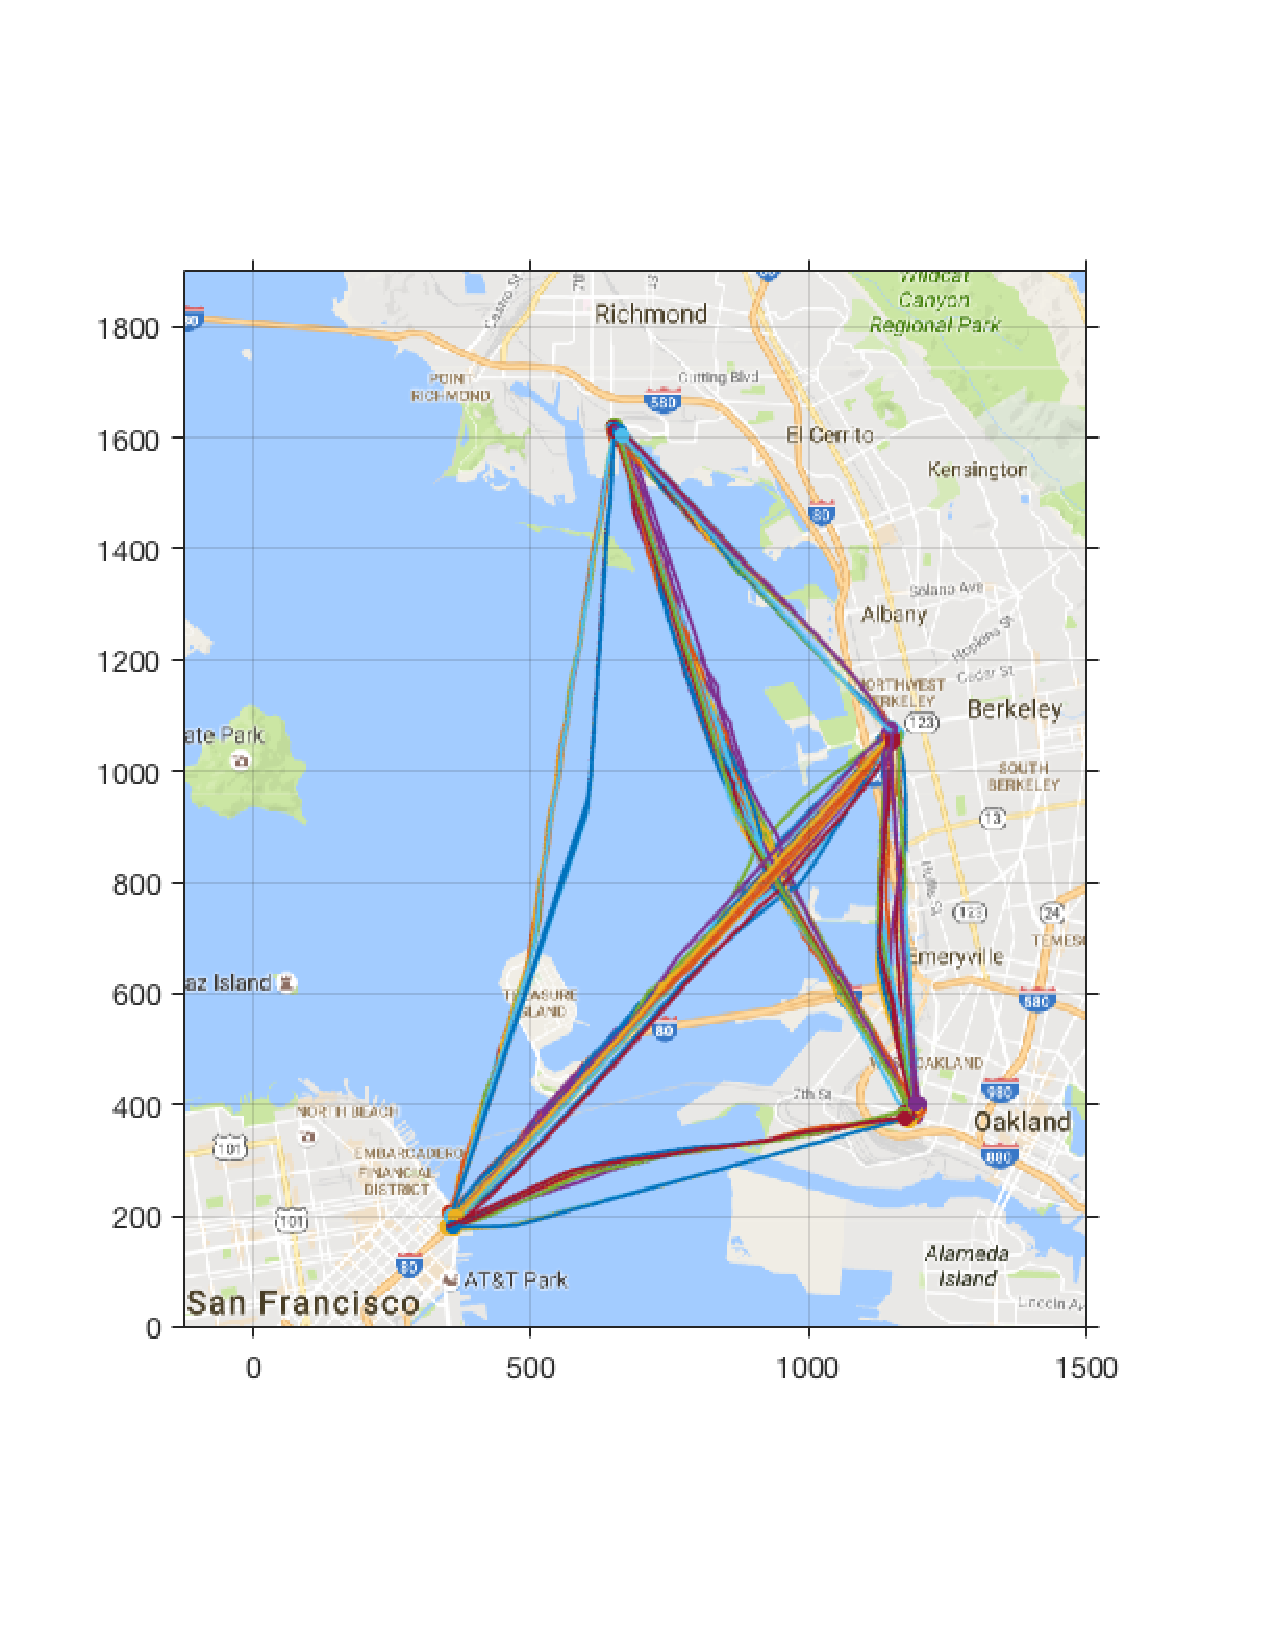
\includegraphics[width=\columnwidth]{figs/bayArea_d11sep5}
  \subcaption{}
  \label{fig:bayArea_d11sep5}
\end{subfigure}%
\begin{subfigure}{\columnwidth}
  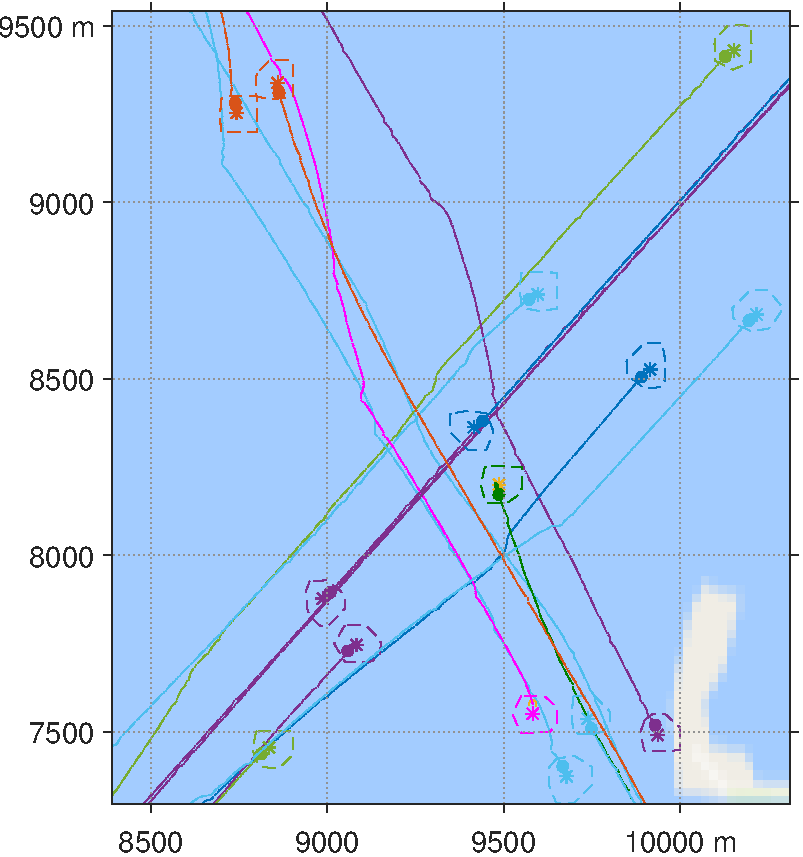
\includegraphics[width=\columnwidth]{figs/bayArea_d11sep5_zoomed}
  \subcaption{}
  \label{fig:bayArea_d11sep5_zoomed}
\end{subfigure}%
  \caption{(a) Trajectories obtained from the SPP algorithm for the multi-city simulation with $d_r = 11m/s$, $\sta_i = 5(i-1)$. (b) Zoomed-in version of the central area. A high density of vehicles is achieved at the center because of the intersection of several trajectories; however, the SPP algorithm still ensures that vehicles do not enter each other's danger zones and reach their destinations.} 
  \label{fig:bayArea_d11sep5_all}
\end{figure*}

Finally, we simulate the system for the case where $\sta_i = 0 ~\forall i$. As evident from Figure \ref{fig:bayArea_d11sep0}, we get multiple lanes between each pair of cities in this case and trajectories become predominately state-separated, as we expect based on the discussion in Section \ref{sec:city_distbEffect}.
\begin{figure}[t]
  \centering
  \includegraphics[width=\columnwidth]{"figs/bayArea_d11sep0"}
  \caption{Vehicle trajectories for $d_r = 11m/s$, $\sta_i = 0$. Since different vehicles have same scheduled times of arrival, a multiple-lane behavior is observed between every pair of cities.} 
  \label{fig:bayArea_d11sep0}
\end{figure}

The average trajectory computation time per vehicle is \SBnote{$XYZ$s} per vehicle on a \SBnote{$Blah Blah$} computing machine. Once again all the computation is done offline and only a lookup table query is required in real-time, which can be performed very efficiently. This simulation illustrates the scalability and the potential of deploying the SPP algorithm for provably safe path planning for large multi-vehicle systems.
% Numerical Simuations (1-1.5p)
%% 2D + 2D example (what example, concretely?
%% Nx3D examples
\section{Numerical Implementation \label{sec:example}}
For the numerical examples in this paper, we use a numerical method provided in \cite{fisac15} which is based on methods in \cite{mitchell05, sethian96}. The numerical algorithm is shown in Algorithm \ref{alg:HJI}. Here, $\mathbf{i}$ represents the index for a particular grid cell, $I$ represents the set of grid indices, and $k$ represents the time step.  $\hat{V}$ represents the numerical approximation to $V$. $D^+_x\hat{V}, D^-_x\hat{V}$ represent the ``right" and ``left" approximations of spatial derivatives. For the numerical Hamiltonian $\hat{H}$, we used the well-known Lax-Friedrich approximation \cite{mitchell-thesis, osher91}.

For spatial derivatives $D^\pm_x\hat{V}$, we used a fifth-order accurate weighted essentially nonoscillatory scheme \cite{osher91,osher03}. For time derivative $D_t \hat{V}$, we used a third-order total variation diminishing Runge-Kutta scheme \cite{osher03, shu88}. For these derivative approximations, the implementation in \cite{LSToolbox} was used. For two-, three-, and four-dimensional (2D, 3D, 4D) computations, we used a $200^2, 71^3, 45^4$ grid, respectively.

\begin{algorithm}[h] 
\KwData{$\hat{l}(x_\mathbf{i},t_\mathbf{k}), \hat{g}(x_\mathbf{i},t_\mathbf{k})$}
 \KwResult{$\hat{V}(x_\mathbf{i},t_\mathbf{k})$}
 \BlankLine
 Initialization\DontPrintSemicolon\;\PrintSemicolon
   \For{$\mathbf{i}\in I$}{
     \nlset{Init}
     $\hat{V}(x_\mathbf{i},t_0) \leftarrow \max\{\hat{l}(x_\mathbf{i},t_0), \hat{g}(x_\mathbf{i},t_0)\}$\;
   }
   Value propagation\DontPrintSemicolon\;\PrintSemicolon
  \For{$k\leftarrow 1$ \KwTo $n$}{
     \For{$\mathbf{i}\in I$}{
     $\hat{V}(x_\mathbf{i},t_k) \leftarrow \hat{V}(x_\mathbf{i},t_{k-1})$ \DontPrintSemicolon\;\PrintSemicolon$\quad+\displaystyle\int_{t_k}^{t_{k-1}} \!\!\!\hat{H}\big(x_\mathbf{i}, D^+_x\hat{V}(x_\mathbf{i},\tau), D^-_x\hat{V}(x_\mathbf{i},\tau)\big)d\tau$\;
$\hat{V}(x_\mathbf{i},t_k) \leftarrow \min \left\{\hat{V}(x_\mathbf{i},t_k), l(x_\mathbf{i},t_k)\right\}$\;
$\hat{V}(x_\mathbf{i},t_\mathbf{k}) \leftarrow \max\left\{\hat{V}(x_\mathbf{i},t_k), g(x_\mathbf{i},t_k)\right\}$\;
     }
   }
 \caption{Numerical Double-Obstacle HJI Solution\label{alg:HJI}}
\end{algorithm}

Note that although the two examples we present have two and four vehicles, our method can be used for \textit{any} number of vehicles, as long as the state space of each vehicle is less than six dimensions. The computational complexity of our method scales linearly with the number of vehicles, allowing the possibility of performing trajectory planning for a very large number of vehicles.

\section{Two Vehicles with Kinematics Model \label{sec:2vek}}
Consider two vehicles $i = 1,2$ using the simple kinematics model with the following dynamics in $t\in[\tnow_i, \tf_i]$:

\begin{equation}
\begin{aligned}
\dotx_i &= v_i\ctrl_i(t), \ctrl_i(t) \in \ctrlin \\
\x_i(\tnow_i) &= \x_i^0 \\
\end{aligned}
\end{equation}

\noindent where $v_1=v_2=1$ are the maximum speeds of the vehicles and $\ctrlin$ is the unit disk. Under this model, each vehicle can move in any direction at some maximum speed. With the above dynamics, the Hamiltonian for each vehicle is

\bq
\ham_i(t, D_{\x_i}\soln_i(\x_i,t), \soln_i(\x_i,t)) = \min_{\ctrl_i} \{v_i\ctrl_i(t) \cdot D_{\x_i}\soln(\x_i, t)\}
\eq

\noindent giving the optimal control 
\bq
\ctrl_i(t) = -\frac{D_{\x_i}\soln_i(\x_i,t)}{\| D_{\x_i}\soln_i(\x_i,t) \|_2}
\eq

The vehicles have the following scheduled times of arrival from the following initial conditions:
\bq
\begin{aligned}
\x_1^0 &= (-0.5, 0), \x_2^0 = (0.5, 0)\\
\tf_1 &= \tf_2 = 0
\end{aligned}
\eq

The target sets of the vehicles are squares with side length $0.2$ on the opposite side of the domain, and the obstacles are rectangles near the middle of the domain. The system's initial conditions and domain are shown in Figure \ref{fig:kin_ic}.

For this system, we determine $\ti_1, \ti_2$, the latest acceptable times that vehicles $1,2$ must depart from their initial positions $\x_1^0, \x_2^0$ in order to reach their respective targets $\target_1, \target_2$ while avoiding obstacles and danger. We will do this by computing the reach-avoid sets from the target sets using two different methods. First, we perform SPP by solving the HJI VI (\ref{eq:HJI}) for the two vehicles as outlined in Section \ref{sec:solution}. Second, note that this system has a 4D joint state space, and thus the single-obstacle HJI VI (\ref{eq:HJIPDE}) would actually be numerically tractable. Therefore, we will also compute the reach-avoid set by solving (\ref{eq:HJIPDE}) in 4D for comparison.

\begin{figure}
	\centering
	\includegraphics[width=0.2\textwidth]{"kin_ic"}
	\caption{Initial configuration of the two-vehicle example.}
	\label{fig:kin_ic}
\end{figure}

\begin{figure}
	\centering
	\includegraphics[width=0.3\textwidth]{"kin_reach"}
	\caption{Evolution of reach-avoid set for vehicle $2$. The initial reach-avoid set at time 0 grows backwards in time unobstructed before it encounters obstacles (left top). Black arrows indicate direction of obstacle motion. When the time reaches $t=-0.61$, the growth of the reach-avoid set is inhibited by both the static obstacle $\obs$ and the time-varying obstacle induced by vehicle 1, $\mobs_1^2$. The evolution of the reach-avoid set is computed until $t=\ti_2=-1.13$, when the reach-avoid set contains vehicle $2$'s initial position.}
	\label{fig:kin_reach}
\end{figure}

\begin{figure}
	\centering
	\includegraphics[width=0.4\textwidth]{"kin_result"}
	\caption{A comparison between the single-obstacle and double-obstacle HJI VI solutions. With the double-obstacle HJI VI solution, vehicle $2$ optimally moves to $\target_2$ while avoiding vehicle $1$, which takes the shortest path to $\target_1$. With the single-obstacle HJI VI solution, both vehicles avoid each other along their way to the targets. The resulting reach-avoid sets at $t=\ti_2$ are very similar in both cases.}
	\label{fig:kin_result}
\end{figure}

\subsection{Solution via double-obstacle HJI VI and SPP}
With the HJI VI and SPP approach, we first determine the minimum time trajectory for vehicle $1$ from $\x_1^0$ to $\target_1$. Then, given this trajectory, we determine the optimal trajectory for vehicle $2$ that brings vehicle $2$ from $\x_2^0$ to $\target_2$ while avoiding the danger zone of vehicle $1$.

Figure \ref{fig:kin_reach} shows the reach-avoid set for vehicle $2$ at various times. We start at $t=\tf_2=0$, and propagate the reach-avoid set backwards in time until $t=\ti_2=-1.13$. Before the induced obstacle touches the reach-avoid set, the reach-avoid set grows from the target set in the same way as in a front propagation problem with uniform speed; this is shown in the left top subplot. Eventually, the obstacle inhibits the propagation of the reach-avoid set, shown in the next two subplots. Finally, the reach-avoid set grows to contain $\x_2^0$, and the computation is stopped at $\ti_2=-1.13$. The left top plot of Figure \ref{fig:kin_result} shows the resulting trajectory from applying the optimal control in Equation (\ref{eq:ctrl_syn}).

Computations were done on a $200^2$ grid. Trajectory planning for vehicle 1 took approximately 0.34 seconds using the fast marching method \cite{sethian96}. Trajectory planning via solving Equation (\ref{eq:HJI}) for vehicle $2$ given the trajectory for vehicle 1 took approximately 25 seconds. Computations were done on a Lenovo T420s laptop with a Core i7-2640M processor, and are orders of magnitude faster than doing a 4D HJI calculation, which took approximately 30 minutes.

\subsection{Solution via single-obstacle HJI VI}
To solve the single-obstacle HJI VI (\ref{eq:HJIPDE}), we define, in the joint state space of the vehicles, the \textit{static} joint target set

\bq
\target = \{(\x_1, \x_2)\in\R^4: \x_1 \in \target_1 \wedge \x_2 \in \target_2 \}
\eq

Next we define, also in the joint state space of the vehicles, the \textit{static} joint avoid set
\bq
\begin{aligned}
\avoid &= \{(\x_1, \x_2)\in\R^4: \x_1 \in \obs \vee \x_2 \in \obs \\
&\qquad \vee \|\x_1-\x_2\|_2\le\Rc \}
\end{aligned}
\eq

Now, we can solve the single-obstacle HJI VI (\ref{eq:HJIPDE}) with the terminal set  $\target\backslash\avoid$, and the avoid set $\avoid$.

The result of solving (\ref{eq:HJIPDE}) is shown in the top right and bottom left subplots of Figure \ref{fig:kin_result}. The top right subplot shows the resulting trajectory, in which the two vehicles cooperatively avoid collision. The bottom left plot compares the reach-avoid sets computed from solving (\ref{eq:HJIPDE}) and the double-obstacle HJI VI (\ref{eq:HJI}) at $t=\ti_2$. The two sets are quite similar. The discrepancy between the reach-avoid sets is due to the difference in control strategies derived from the two different approaches: with the single-obstacle HJI VI, we compute the joint optimal control for both vehicles, and with the double-obstacle HJI VI, we compute the optimal control for vehicle 2 given vehicle 1's optimal trajectory, which does not take into account vehicle 2's motion. 

For the latest start time, we obtained $\ti_2 = -1.15$ from the single-obstacle HJI VI (recall $\ti_2=-1.13$ from the double-obstacle HJI VI). This discrepancy is likely due to the grid resolution limitation when doing a 4D calculation. Computations were done on a $45^4$ grid, and took approximately 30 minutes.

\section{Four Vehicles with Constrained Turn Rate}
Consider four vehicles with states $\x_i = [x_i, y_i, \theta_i]^\top$ modeled using a horizontal kinematics model with the following dynamics for $t \in[\tnow_i, \tf_i],i=1,2,3,4$:

\begin{equation}
\begin{aligned}
\dot{x}_i &= v_i \cos(\theta_i) \\
\dot{y}_i &= v_i \sin(\theta_i) \\
\dot{\theta}_i &= \omega_i \\
\x_i(\tnow_i) &= \x_i^0 \\
|\omega_i| &\le \bar{\omega}_i \\
\end{aligned}
\end{equation}

\noindent where $(x_i, y_i)$ is the position of vehicle $i$, $\theta_i$ is the heading of vehicle $i$, and $v_i$ is the speed of vehicle $i$. The control input $\ctrl_i$ of vehicle $i$ is the turning rate $\omega_i$, whose absolute value is bounded by $\bar{\omega}_i$. For illustration, we chose $\bar{\omega}_i=1 \forall i$ and assume $v_i=1$ is constant; however, our method can easily handle the case in which $\bar{\omega}_i$ differ across vehicles and $v_i$ is a control input. The Hamiltonian associated with vehicle $i$ is

\bq
\begin{aligned}
\ham_i(t, &D_{\x_i}\soln_i(\x_i,t), \soln_i(\x_i,t)) \\
&= \min_i \big\{ v_i D_{x_i} \soln_i(\x_i, t) \cos(x_i(t)) \\
&\; + v_i D_{y_i} \soln_i(\x_i, t) \sin(y_i(t)) + D_{\theta_i} \soln_i(\x_i, t) \omega_i \big\}
\end{aligned}
\eq

\noindent giving the optimal control
\bq
\omega_i(t) = -\bar{\omega}_i\frac{D_{\theta_i}\soln_i(\x_i,t)}{\left| D_{\theta_i}\soln_i(\x_i,t) \right|}
\eq

The vehicles have initial conditions and STA as follows:
\bq
\begin{aligned}
\x_1^0 &= (-0.5, 0, 0), &\tf_1 &= 0\\
\x_2^0 &= (0.5, 0, \pi), &\tf_2 &= 0.2\\
\x_3^0 &= \left(-0.6, 0.6, \frac{7\pi}{4}\right), &\tf_3 &= 0.4\\
\x_4^0 &= \left(0.6, 0.6, \frac{5\pi}{4}\right), &\tf_4 &= 0.6\\
\end{aligned}
\eq

The target sets $\target_i$ of the vehicles are all 4 circles of radius $0.1$ in the domain. The centers of the target sets are at $(0.7, 0.2), (-0.7, 0.2), (0.7, -0.7), (-0.7, -0.7)$ for vehicles $i=1,2,3,4$, respectively. The domain $\amb$ and obstacles $\obs$ are the same as those of the example in Section \ref{sec:2vek}. The setup for this example is shown in Figure \ref{fig:dubins_ic}. 

The joint state space of this system is twelve-dimensional, intractable for analysis using the single-obstacle HJI VI (\ref{eq:HJIPDE}). Therefore, we will repeatedly solve the double-obstacle HJI VI (\ref{eq:HJI}) to compute the reach-avoid sets from targets $\target_i$ for vehicles $1,2,3,4$, in that order, with moving obstacles induced by vehicles $j=1,\ldots,i-1$. We will also obtain $\ti_i,i=1,2,3,4$, the LSTs for each vehicle in order to reach $\target_i$ by $\tf_i$.

Figures \ref{fig:dubins_reach_all}, \ref{fig:dubins_reach_3}, and \ref{fig:dubins_result} show the results. Since the state space of each vehicle is 3D, the reach-avoid set is also 3D. To visualize the results, we slice the reach-avoid sets at the initial heading angles $\theta_i^0$. Figure \ref{fig:dubins_reach_all} shows the 2D reach-avoid set slices for each vehicle at its LSTs $\ti_1=-1.12, \ti_2=-0.94,\ti_3=-1.48,\ti_4=-1.44$ determined from our method. The obstacles in the domain $\obs$ and the obstacles induced by other vehicles inhibit the evolution of the reach-avoid sets, carving out thin ``channels" that separate the reach-avoid set into different ``islands". One can see how these channels and islands form by looking at the time evolution of the reach-avoid set, shown in Figure \ref{fig:dubins_reach_3} for vehicle 3. 

Finally, Figure \ref{fig:dubins_result} shows the resulting trajectories of the four vehicles. The subplot labeled $t=-0.55$ shows all four vehicles in close proximity without collision: each vehicle is outside of the danger zone of all other vehicles. The actual arrival times of vehicles $i=1,2,3,4$ are $0, 0.19, 0.34, 0.31$, respectively. It is interesting to note that for some vehicles, the actual arrival times are earlier than the STAs $\tf_i, i=1,2,3,4$. This is because in order to arrive at the target by $\tf_i$, these vehicles must depart early enough to avoid major delays  resulting from the induced obstacles of other vehicles; these delays would have lead to a late arrival if vehicle $i$ departed after $\ti_i$.

\begin{figure}
	\centering
	\includegraphics[width=0.275\textwidth]{"dubins_ic"}
	\caption{Initial configuration of the four-vehicle example.}
	\label{fig:dubins_ic}
\end{figure}

\begin{figure}
	\centering
	\includegraphics[width=0.4\textwidth]{"dubins_reach_all"}
	\caption{Reach-avoid sets at $t=\ti_i$ for vehicles $1,2,3,4$, sliced at initial headings $\theta_i^0$. Black arrows indicate direction of obstacle motion. Due to the turn rate constraint, the presence of static obstacles $\obs$ and time-varying obstacles induced by higher-priority vehicles $\mobs^i_j(t)$ carves ``channels" in the reach-avoid set, dividing it up into multiple ``islands".}
	\label{fig:dubins_reach_all}
\end{figure}

\begin{figure}
	\centering
	\includegraphics[width=0.4\textwidth]{"dubins_reach_3"}
	\caption{Time evolution of the reach-avoid set for vehicle $3$, sliced at its initial heading $\theta_3^0=\frac{7\pi}{4}$. Black arrows indicate direction of obstacle motion. Initially, the reach-avoid set grows unobstructed by obstacles, as shown in the top subplots. Then, in the bottom subplots, the static obstacles $\obs$ and the induced obstacles of vehicles $1$ and $2$, $\mobs^3_1,\mobs^3_2$, carve out ``channels" in the reach-avoid set.}
	\label{fig:dubins_reach_3}
\end{figure}

\begin{figure}
	\centering
	\includegraphics[width=0.4\textwidth]{"dubins_result"}
	\caption{The planned trajectories of the four vehicles. In the left top subplot, only vehicles $3$ (green) and $4$ (purple) have started moving, showing $\ti_i$ is not common across the vehicles. Right top subplot: all vehicles have come within very close proximity, but none is in the danger zone another. Left bottom subplot: vehicle $1$ (blue) arrives at $\target_1$ at $t=0$. Right bottom subplot: all vehicles have reached their destination, some ahead of the STA $\tf_i$.}
	\label{fig:dubins_result}
\end{figure}

% % !TEX root = STP_journal.tex
\section{Conclusions and Future Work}
Guaranteed-safe multi-vehicle trajectory planning is a challenging problem, and previous analyses often either require strong assumptions on the motion of the vehicles or result in a large degree of conservatism. Differential game techniques such as Hamilton-Jacobi (HJ) reachability are ideally suited for guaranteeing goal satisfaction and safety under disturbances, but become intractable for even a small number of vehicles.

Our robust sequential trajectory planning (STP) method assigns a strict priority ordering to vehicles to offer a tractable and practical approach to the multi-vehicle trajectory planning problem. Under the proposed method, a portion of ``space-time'' is reserved for vehicles in the airspace in descending priority order to allow for dense vehicle configurations. Unlike previous priority-based methods, our approach accounts for disturbances and an adversarial intruder. STP reduces the scaling of HJ reachability's computational complexity from exponential to linear with respect to the number of vehicles, while maintaining hard guarantees on goal satisfaction and safety under disturbances. In the presence of a single intruder vehicle, STP still guarantees goal satisfaction and safety with a quadratically scaling computational complexity.

In the future, we plan to investigate ways of guaranteeing a maximum number of vehicles that need to re-plan, combine reachability analysis with other trajectory and path planning methods to improve computation speed, and to better understand the scenarios under which the STP scheme is the most useful by running large-scale simulations.
\vspace{-0.2cm}
% Conclusion (0.5p)
\section{Conclusions and Future Work}
We have presented a problem formulation that allows us to consider the multi-vehicle trajectory planning problem in a tractable way by planning trajectories for vehicles in order of priority. In order to do this, we modeled higher-priority vehicles as time-varying obstacles. We then solved a double-obstacle HJI VI to obtain the reach-avoid set for each vehicle. The reach-avoid set characterizes the region from which each vehicle is guaranteed to arrive at its target within a time horizon, while avoiding collision with obstacles and higher-priority vehicles. The solution also gives each vehicle a latest start time as well as the optimal control which guarantees that each vehicle safely reaches its target on time. This paper provides a first application of the double-obstacle HJI VI. Immediate future work includes investigating ways to relax assumptions about the knowledge of the trajectories of other vehicles, more sophisticated induced obstacles for modeling trajectory uncertainty, and problems involving adversarial agents, among many other possibilities.

%%%%%%%%%%%%%%%%%%%%%%%%%%%%%%%%%%%%%%%%%%%%%%%%%%%%%%%%%%%%%%%%%%%%%%%%%%%%%%%%
%\addtolength{\textheight}{1cm}   % This command serves to balance the column lengths
                                  % on the last page of the document manually. It shortens
                                  % the textheight of the last page by a suitable amount.
                                  % This command does not take effect until the next page
                                  % so it should come on the page before the last. Make
                                  % sure that you do not shorten the textheight too much.

\bibliographystyle{IEEEtran}
\bibliography{references}
\end{document}
